\section{Problem Formulation}


In this section, we provide the formal definition of graph window query.
%In this section, we provide the formal definition of graph window query. 
We use $G = (V,E)$ to denote a directed/undirected data graph, where $V$ is its vertex set and $E$ is its edge set.
Each node/edge is associated with a (possibly empty) set of attribute-value pairs.

%\begin{defn}
%\label{attributed_graph}
%[Attributed Graph]
%Let $G = (V,E,A)$ be an attribute graph, where $V$ is  its vertex set, $E$ is its edge set and $A$ is its attribute set respectively. An edge $e(u,v) \in E$ indicates that $u$ is linked to $v$, where $u \in V$ and $v \in V$. For every vertex in the graph, there exists one multidimensional vector in $A$ representing the attributes of the vertex. i.e. $\forall v \in V, \exists a(v)=(a_1,a_2..,a_k) \in A$.
%\end{defn} 

Figure~\ref{fig:attributed} shows an undirected graph representing a social network that we will use as our running example in this paper. 
The table shows the values of the five attributes (User, Age, Gender, Industry, and Number of posts) associated with each vertex. For convenience, each node is labeled with its user attribute value;
and there is one edge between a user X and another user Y if X and Y are connected in the social network.


\begin{figure}[h]
\centering
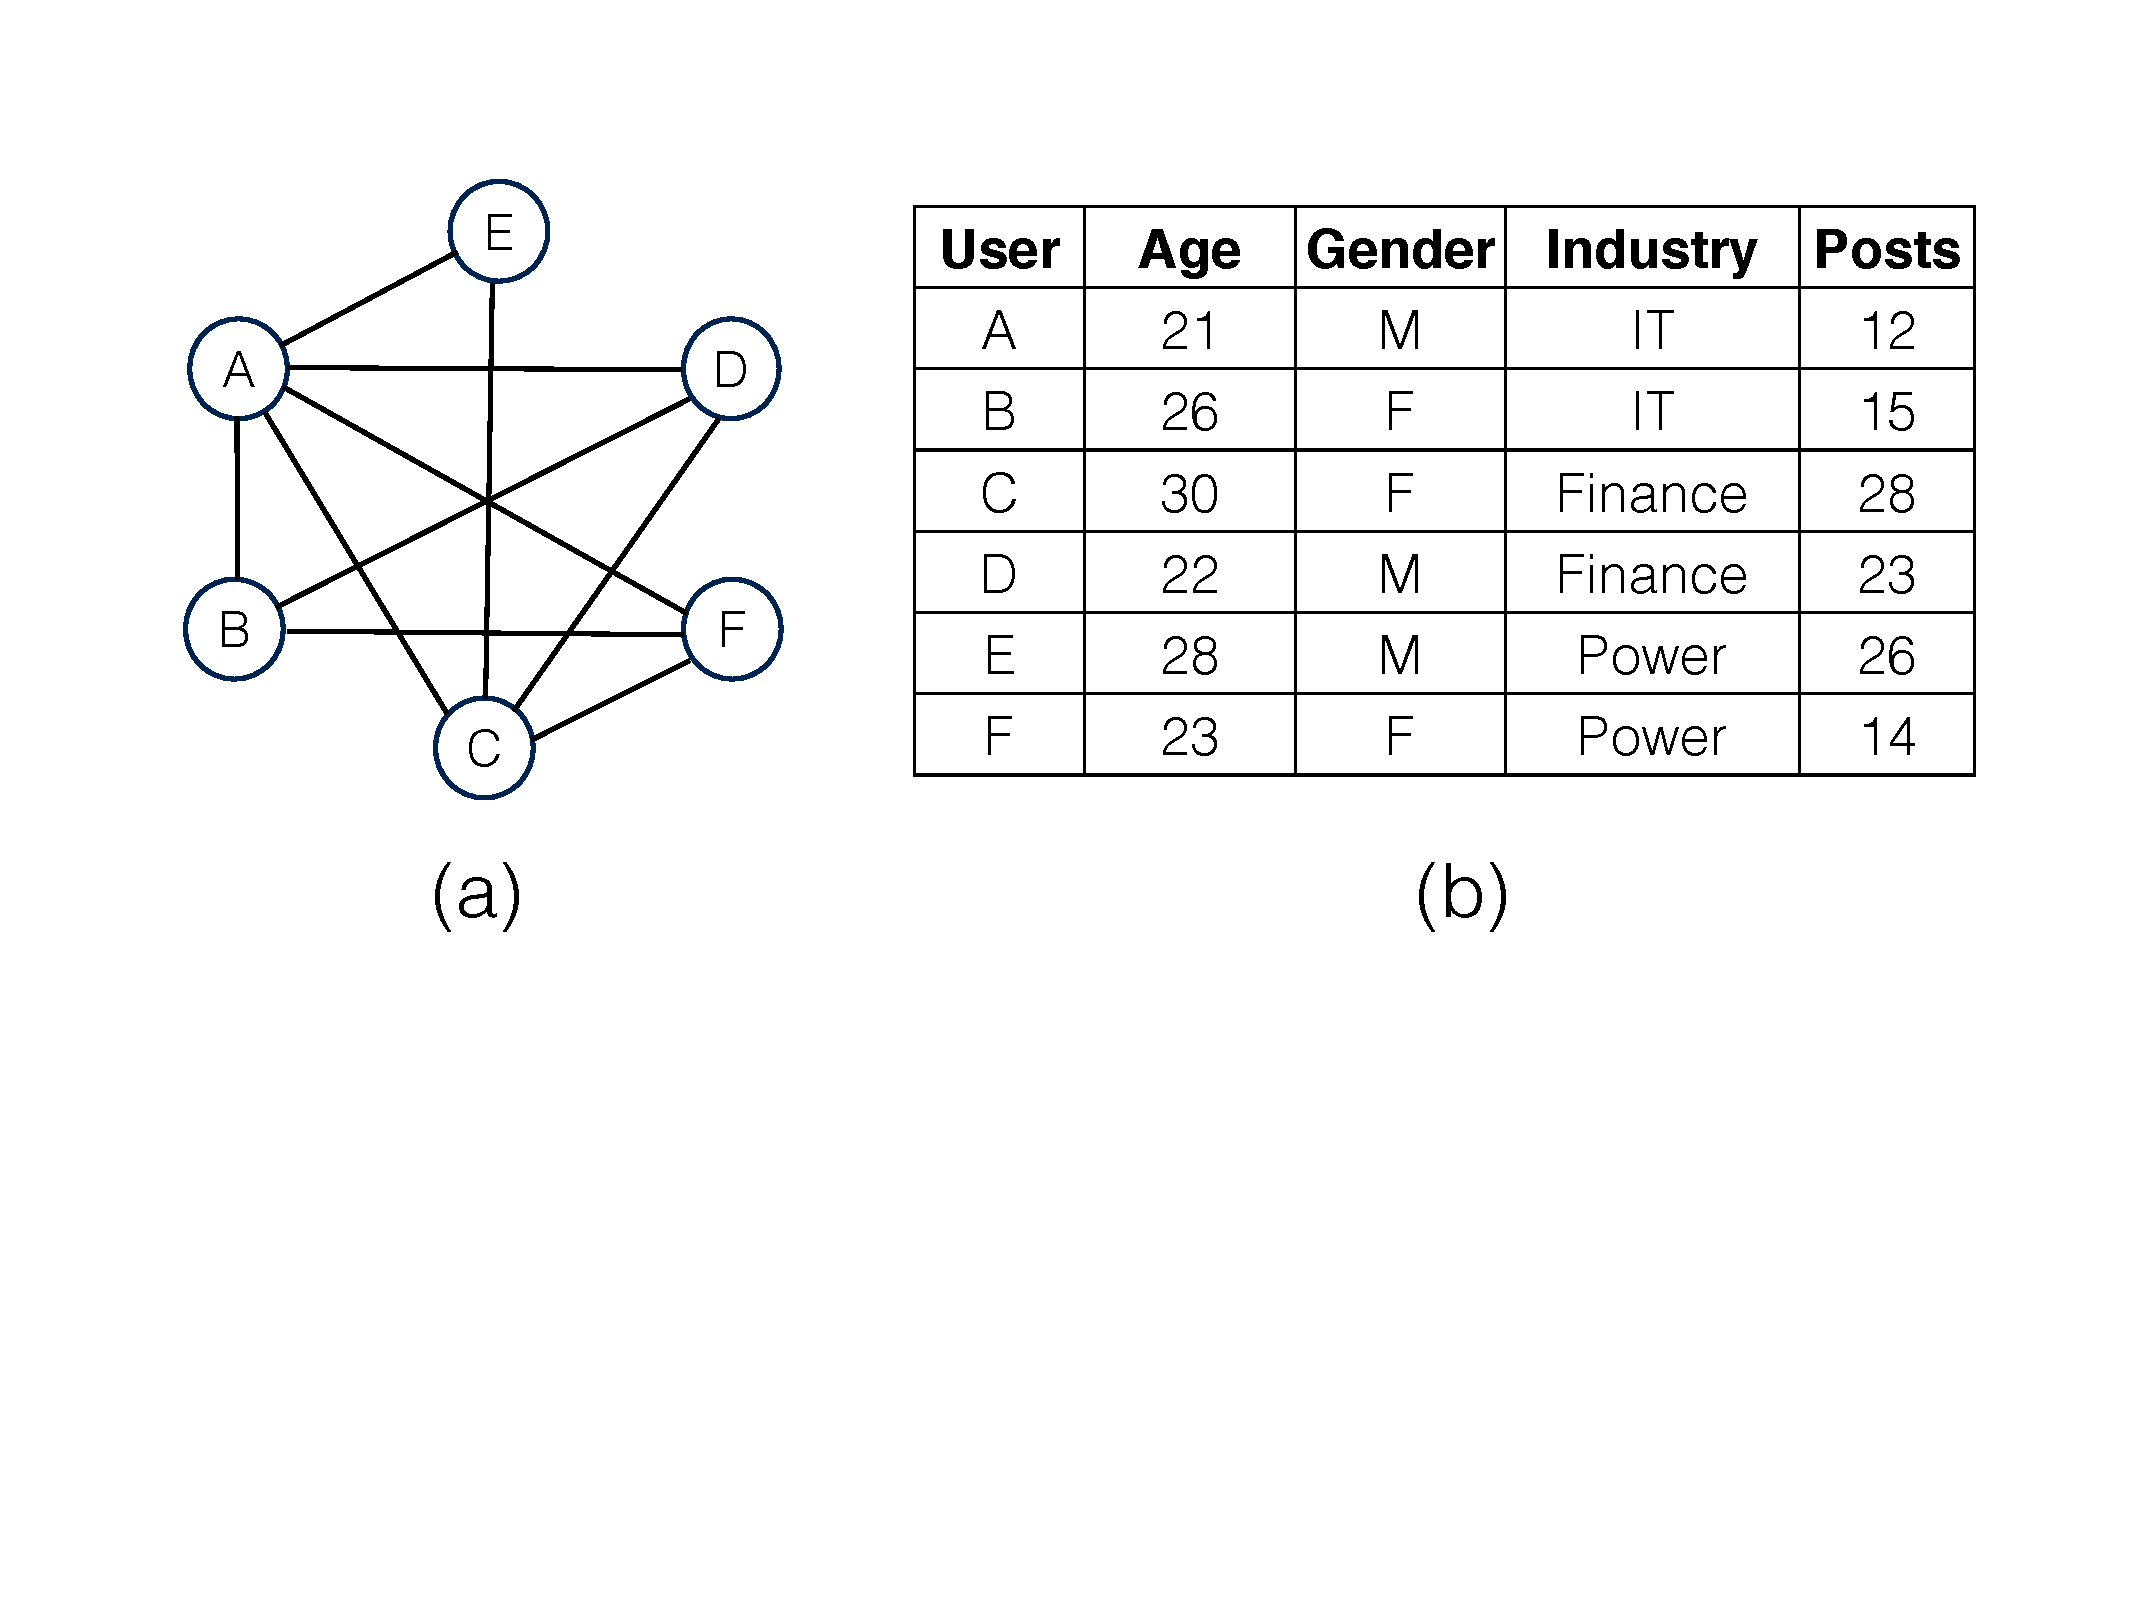
\includegraphics[width=0.8\textwidth]{chapter3/attributed_graph.pdf}
	\caption{A miniature social graph. (a) the graph structure; (b) the attributes associated with the vertexes of (a).} 
	\label{fig:attributed}
\end{figure}

Given a data graph $G = (V,E)$,
a \emph{Graph Window Function (GWF)} over $G$ can be expressed 
as a quadruple $(G, W, \Sigma, A)$, where 
$W(v)$ denotes a \emph{window specification} for a vertex $v \in V$ 
that determines the set of vertices in some subgraph of $G$,
$\Sigma$ denotes an \emph{aggregation function}, and $A$ denotes 
a \emph{vertex attribute}.
The evaluation of a GWF $(G, W, \Sigma, A)$ on $G$
computes for each vertex $v$ in $G$, the aggregation $\Sigma$ on the 
values of attribute $A$  
over all the vertices in $W(v)$, which we denote by $\Sigma_{v' in W(v)} v'.A$.

Note that, in this paper, we focus on the attribute-based aggregation with distributive or algebraic aggregation functions. 
In other words, $W(v)$ refers to a set of vertices, and the aggregation function 
$\Sigma$ operates on the values of attribute $A$ over all the vertices in $W(v)$. Meanwhile, the aggregation function $\Sigma$ is distributive or algebraic (e.g., sum, count, average), as these aggregation functions are widely used in practice. 
 
In the following, we introduce two useful types of window specification (i.e., $W$), namely, 
\emph{k-hop window} and \emph{topological window}.


\begin{definition}[$k$-hop Window] 
Given a vertex $v$ in a data graph $G$, 
the $k$-hop window of $v$, denoted by $W_{kh}(v)$ (or $W(v)$ when there is no ambiguity),
is the set of neighbors of $v$ in $G$ which can be reached within $k$ hops.
For an undirected graph $G$,
a vertex $u$ is in $W_{kh}(v)$  iff there is a $\alpha$-hop path between $u$ and $v$ where $\alpha \leqslant k$.
For a directed graph $G$,
a vertex $u$ is in $W_{kh}(v)$  iff there is a $\alpha$-hop directed path from $v$ to $u$ \footnote{
Other variants of k-hop window for directed graphs are possible; e.g.,
a vertex $u$ is in $W_{kh}(v)$  iff there is a $\alpha$-hop directed path from $u$ to $v$ where $\alpha \leqslant k$.
} where $\alpha \leqslant k$.
\end{definition}

Intuitively, a k-hop window selects the neighboring vertices of a 
vertex within a  k-hop distance. 
These neighboring vertices typically represent the most important 
vertices to a vertex with regard to their structural relationship in a graph. 
Thus, k-hop windows provide meaningful specifications for many applications, such as customer behavior analysis \cite{briscoe2013determining,dai2012predicting} , digital marketing \cite{ma2010ego} etc.
%\remark{Cite some papers here to justify.}

As an example, in Figure~\ref{fig:attributed}, the $1$-hop window of vertex \emph{E} is $\{A,C,E\}$ and the $2$-hop window of vertex \emph{E} is $\{A,B,C,D,E,F\}$.  

\begin{definition}[Topological Window] 
Given a vertex $v$ in a DAG $G$, the topological window of $v$, denoted by $W_t(v)$,
refers to the set of ancestor vertices  of $v$ in $G$;
i.e., a vertex $u$ is in $W_t(v)$ iff there is directed path from $u$ to $v$ in $G$.
\end{definition}

There are many directed acyclic graphs (DAGs) in real-world applications (such as biological networks, citation networks and dependency networks)
where topological windows represent meaningful relationships that are of interest.
For example, in a citation network where (X,Y) is an edge  iff paper $X$ cites paper $Y$, 
the topological window of a paper represents the citation impact of that paper \cite{campanario2011empirical,holsapple2003citation,ma2008bringing}.

As an example, Figure~\ref{fig:topological} shows a small example of a Pathway Graph from a biological network. 
The topological window of $E$ $W_t(E)$ is $\{A, B, C, D, E\}$ and $W_t(H)$ is $\{A, B, D, H\}$.


\begin{figure}[h]
\centering
 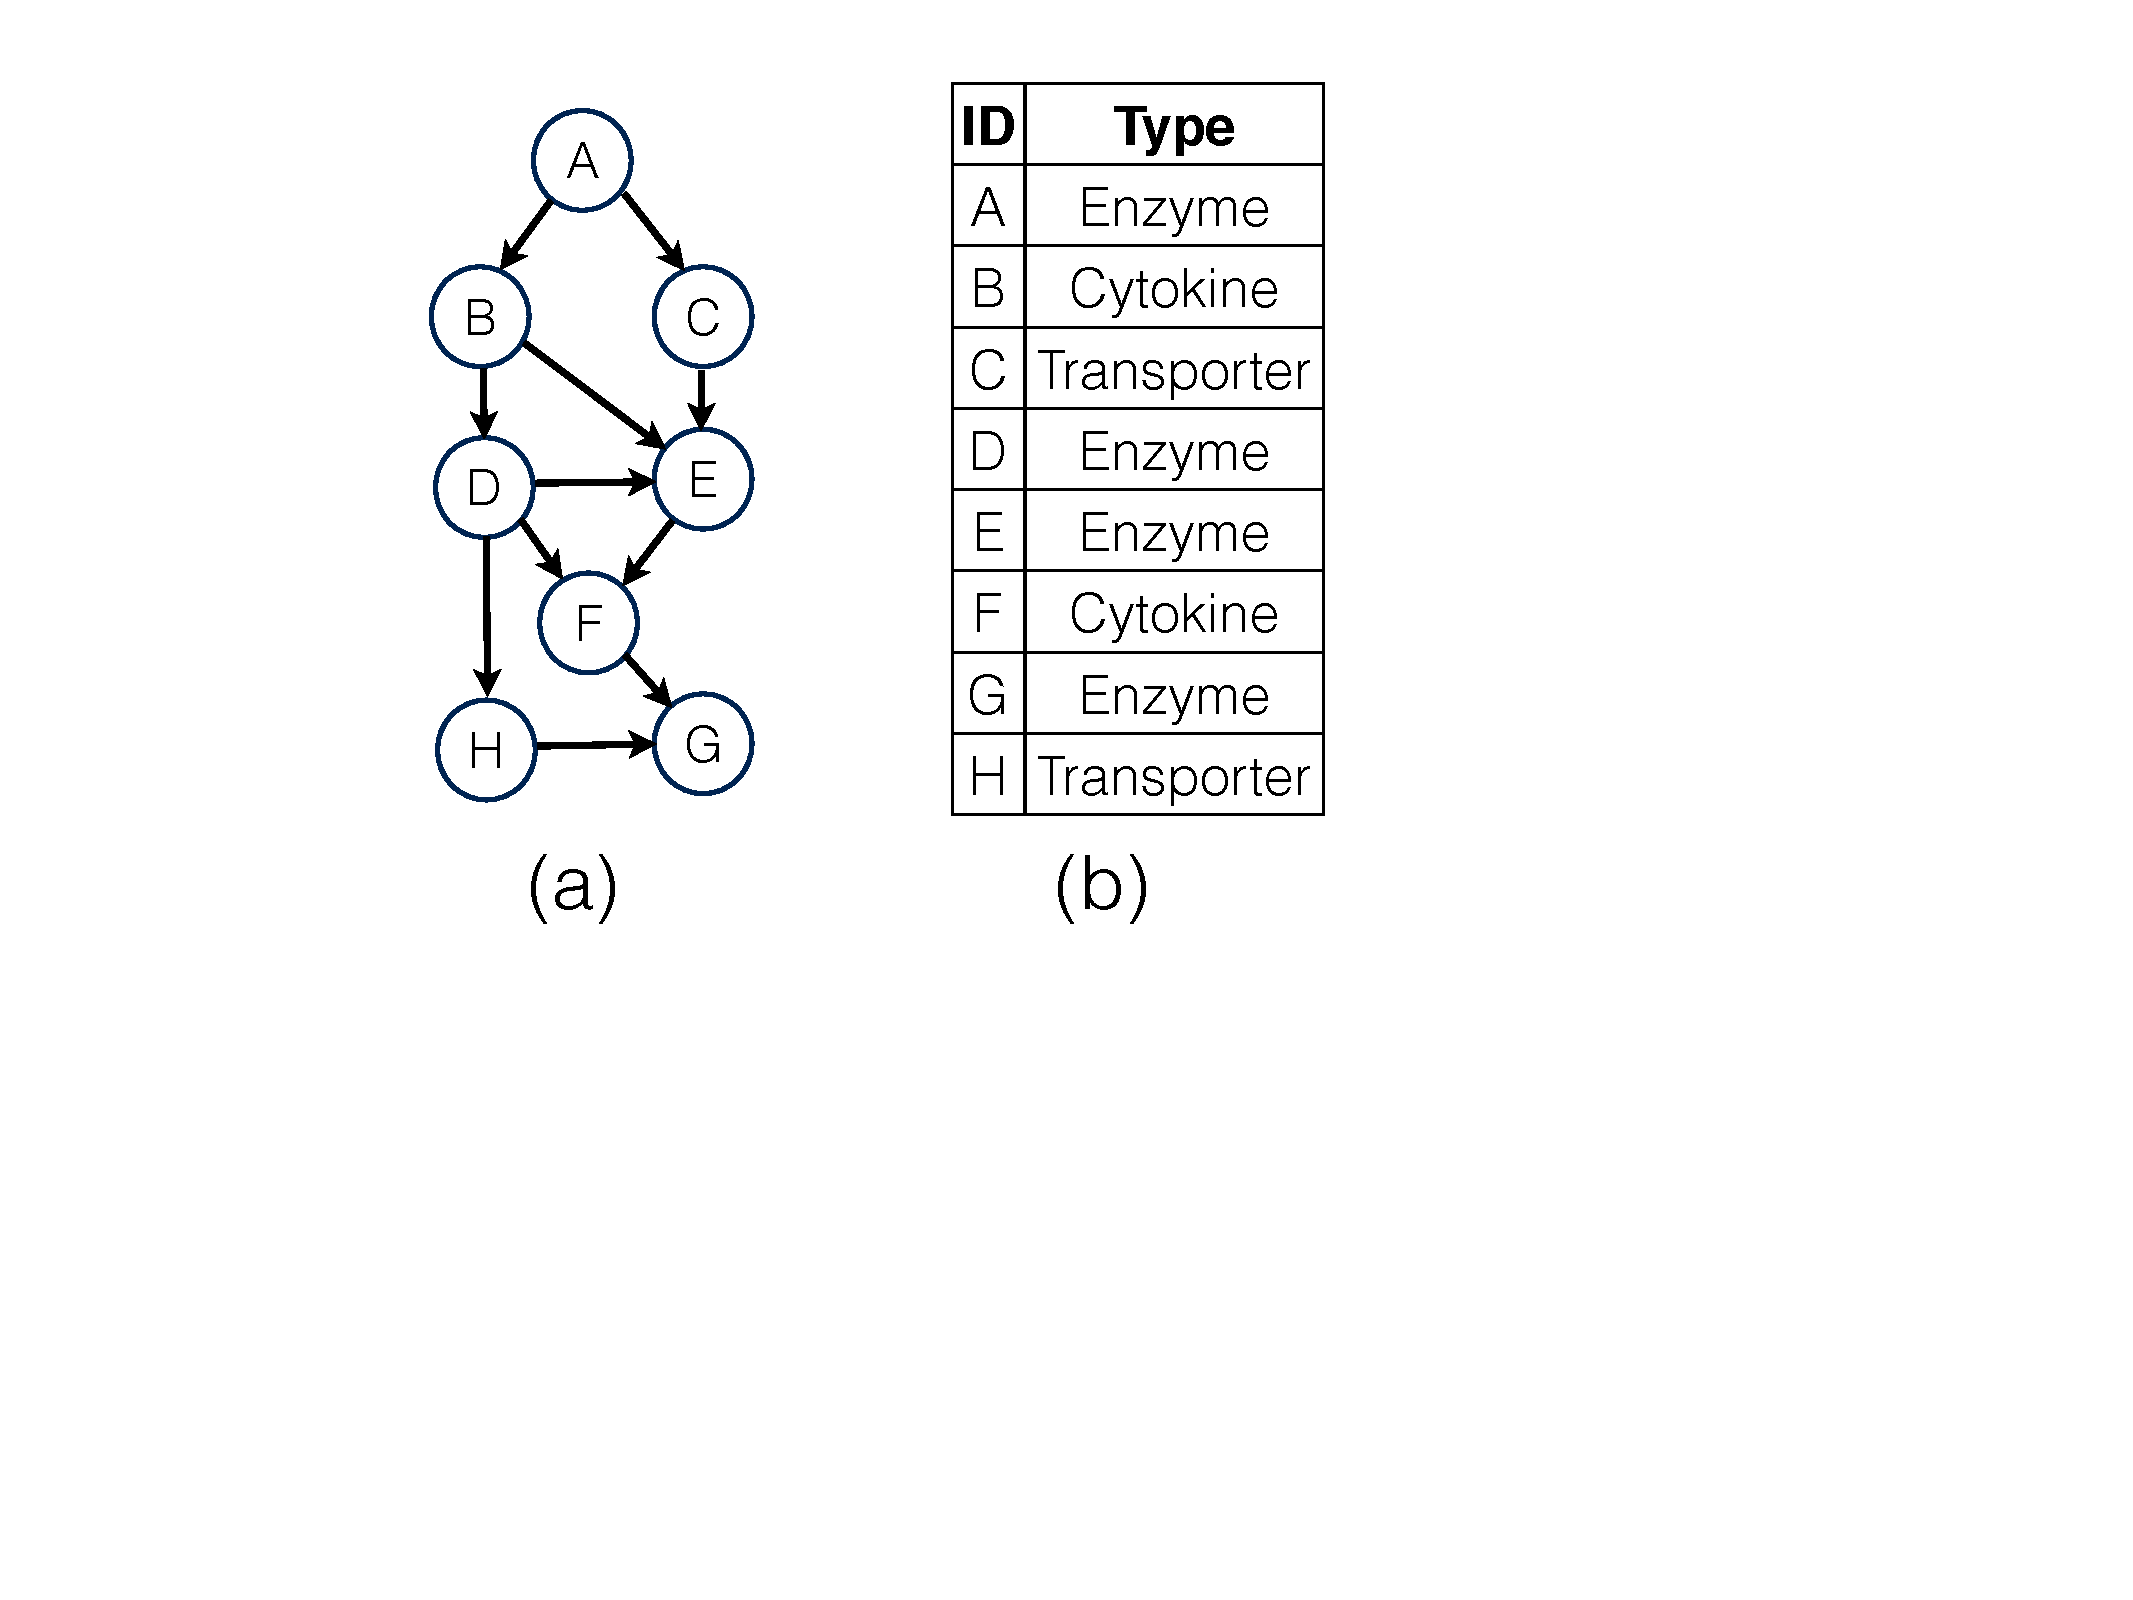
\includegraphics[width=0.8\textwidth]{chapter3/dag.pdf}
	\caption{A miniature pathway DAG. (a) the DAG structure; (b) the attributes associated with the vertexes of (a).}
	\label{fig:topological}
\end{figure}

\begin{definition}[Graph Window Query] 
A graph window query on a data graph $G$ is of the form
$GWQ(G, W_1, \Sigma_1, A_1,\cdots,$ \\
$W_m, \Sigma_m, A_m)$, where $m \geq 1$
and
each quadruple $(G, W_i,\Sigma_i,A_i)$ is a graph window function on $G$.
\end{definition}
In this paper, we focus on graph window queries with a single window 
function that is either a k-hop or topological window. 
The evaluation of complex graph window queries with multiple window 
functions can be naively processed as a sequence of window functions one
after another. 
We leave the optimization of processing multiple
window functions for further study in the future.

